\documentclass[conference]{IEEEtran}
\usepackage{graphicx}
\usepackage{url}
\usepackage{booktabs}
\usepackage{amsmath}
\usepackage[hidelinks]{hyperref}
\graphicspath{{../results/figures/}{hardware/}}

% Small helper for compact tables
\newcommand{\tsmall}{\footnotesize\setlength{\tabcolsep}{3.5pt}}

\begin{document}

\title{Optimizing a Low-Cost Wrist Heart-Rate Sensor\\
with PPG, Motion Data and Machine Learning}

\author{\IEEEauthorblockN{Joe Neglia}
\IEEEauthorblockA{University of Colorado Boulder\\
Boulder, CO, USA\\
jone2220@colorado.edu}}

\maketitle

\begin{abstract}
Can you cheaply build a wearable that tells you your heart rate with reasonable accuracy? I built a wrist band from hobbyist parts, with an optical pulse sensor and a motion sensor, and compared it with a chest strap. A two-stage model first recognises the activity from the motion sensor and then estimates heart rate. When the wearer is resting it uses the frequency of the pulse signal, and otherwise it uses a gradient-boosting model. On a held-out test session the typical error is 9.69~BPM, compared with 34.24~BPM for the declared baseline and 11.14~BPM for a simple per-activity average. The error is only 2.3~BPM when the wearer is still, but 13.5~BPM while walking or running, where the band reads more than 10~BPM too low in 39\% of windows. The answer is yes for rest and desk work, and not yet for exercise.
\end{abstract}

{\raggedright\noindent\textbf{Repository:} \url{https://github.com/JoeNeglia/Fitness_Band}, folder \texttt{fitband-ml}. The README lists every command. \texttt{python analysis/final.py} reproduces the headline number. The seed is fixed at 42 and all data is included.\par}

% =============================================================================
\section{The Question and the Decision}
% =============================================================================
Commercial fitness watches estimate heart rate from light shone into the wrist. This signal is called photoplethysmography, or PPG. It works well when the wrist is still, but arm movement adds noise that can be larger than the pulse itself. The practical question of this project is whether a cheap home-built band, helped by machine learning, can give a heart rate accurate enough to rely on.

\textbf{The decision.} I am both the builder and the wearer. For each activity, I decide whether to trust the band's heart rate or keep wearing a Garmin HRM~200 chest strap, which serves as the ground truth.

\textbf{Why accuracy matters.} Heart rate is rarely used on its own. Wearables build many other health measures on top of it, such as sleep scores, resting heart-rate trends, recovery or readiness scores, calories burned and training zones. An error in heart rate flows into all of them, so an accurate reading is the base for understanding someone's general health.

\textbf{The cost of each error.}
\begin{itemize}
\item \emph{Reading too low during exercise} is the costly error. The wearer thinks they are working less hard than they are and may push into overexertion. For someone with a heart condition this is a safety issue.
\item \emph{Reading too high during exercise} makes the wearer back off for no reason. The cost is a less effective workout, not harm.
\item \emph{Errors at rest} are cheap when small. But a band that simply reports the usual resting value would hide a real change, and it would corrupt measures such as sleep score that depend on resting heart rate. The method has to actually measure the pulse.
\end{itemize}
Besides RMSE, I therefore report the share of windows within 5 and 10~BPM of the truth and the share that read more than 10~BPM too low. As a working rule, an activity is good enough if RMSE is at most 5~BPM and fewer than 10\% of windows read more than 10~BPM too low. This rule was not in the proposal. I set it while writing this report, and the recommendation does not depend on its exact values.

% =============================================================================
\section{The Device and the Data}
% =============================================================================
\textbf{Hardware.} The prototype, shown in Fig.~\ref{fig:prototype}, has three parts on the dominant arm: a MAX30102 PPG sensor against the inside of the wrist, an LSM6DS3 motion sensor board just above it, and a Seeed XIAO nRF52840 board on the forearm, connected by wires and held on with elastic bands. The motion sensor has an accelerometer, which measures movement and wrist angle, and a gyroscope, which measures rotation. Every 100~ms the XIAO sends one line over Bluetooth with the PPG reading and the six motion values. This was a deliberately simple design, meant only to collect data and test whether the idea works, not to be the finished band.

\begin{figure}[t]
\centering
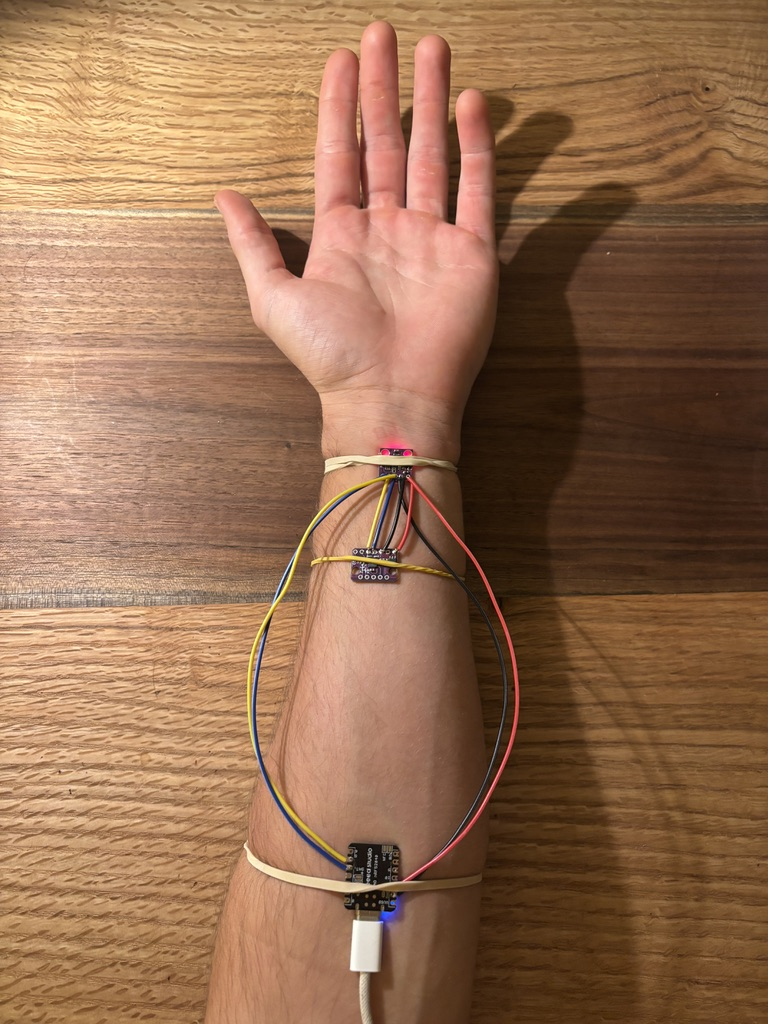
\includegraphics[width=0.55\columnwidth]{prototype.jpeg}
\caption{The proof-of-concept prototype used for all data collection. From the wrist up: the PPG sensor, the motion sensor and the XIAO board.}
\label{fig:prototype}
\end{figure}

\textbf{Collection pipeline.} A laptop script receives the band and the chest strap at the same time and stamps both with the laptop's clock, which lines them up. The strap sends heart rate twice per second plus the time between beats. Each activity is saved as its own CSV file per device.

\textbf{Protocol.} Each session has four 5-minute blocks: resting, typing, walking and running. Sessions 4 and 5 changed the walking and running pace every 100~s, in a different order each time (Table~\ref{tab:sessions}). All sessions were recorded in the same room. The band had to stay near the laptop for reliable Bluetooth, and I did not have a treadmill, so I walked and ran in place and tried to copy my real form as closely as I could.

\begin{table}[t]
\centering\tsmall
\caption{Recording sessions}
\label{tab:sessions}
\begin{tabular}{@{}llll@{}}
\toprule
Session & Date & Walk and run pace & Role \\
\midrule
1--3 & Nov 12, one evening & constant & development \\
4 & Nov 15 & easy, medium, hard & development \\
5 & Nov 15 & medium, hard, easy & \textbf{test, used once} \\
\bottomrule
\end{tabular}
\end{table}

\textbf{Windows and labels.} Each block is cut into 6-second windows that do not overlap, giving 49 to 50 windows per block and 988 in total. The label for a window is the mean chest-strap heart rate. A second label computed from the time between beats agrees within 1.0~BPM on average, so the labels are trustworthy.

\textbf{Features.} Eight signals are summarised by five statistics each, giving 40 features per window (Table~\ref{tab:features}). The 35 motion features describe what the wrist is doing. The 5 PPG features describe the pulse signal.

\begin{table}[t]
\centering\tsmall
\caption{Features: every signal is summarised by every statistic}
\label{tab:features}
\begin{tabular}{@{}lp{0.68\columnwidth}@{}}
\toprule
\multicolumn{2}{@{}l}{\emph{Signals, 8}} \\
\midrule
\texttt{ppg} & Light reflected from the wrist. It rises and falls with each heartbeat. \\
\texttt{ax, ay, az} & Acceleration along three axes: how the wrist moves and which way it points. \\
\texttt{gx, gy, gz} & Rotation speed around three axes. \\
\texttt{acc\_mag} & Total acceleration, $\sqrt{a_x^2+a_y^2+a_z^2}$, which ignores wrist angle. \\
\midrule
\multicolumn{2}{@{}l}{\emph{Statistics, 5}} \\
\midrule
\texttt{mean} & Average level. For \texttt{ay} it shows the wrist angle. For \texttt{ppg} it shows how well the sensor touches the skin. \\
\texttt{std} & Spread around the mean: how much the signal moves. \\
\texttt{skew} & Lopsidedness: are the spikes mostly upward or downward? \\
\texttt{kurt} & How spiky the signal is compared with a smooth wave. \\
\texttt{energy} & Strength of the signal between 0.5 and 3~Hz, which covers both heartbeats and arm swing. \\
\bottomrule
\end{tabular}
\end{table}

% =============================================================================
\section{Method}
% =============================================================================
\textbf{Testing on unseen sessions.} Neighbouring windows are almost copies of each other, so a random split would test the model on windows it has nearly seen. Instead, development uses sessions 1--4 and holds out one whole session at a time: train on three, test on the fourth, and repeat four times. This is called leave-one-session-out. Session 5 is the final test. The data loader refuses to give its rows to any script except \texttt{final.py}, which ran once after every choice was frozen.

\textbf{Error measure.} Heart-rate error is the root-mean-square error, RMSE, in BPM. It is roughly the typical size of a miss, with large misses counted more heavily. Activity recognition is scored with macro-F1, which gives every activity equal weight.

\subsection{Baseline: the FFT of the pulse signal}
The declared baseline is the standard signal-processing estimate. The PPG is filtered to keep 0.67--3.5~Hz, which is 40--210~BPM. A Fourier transform then shows how strong each frequency is in the window, and the strongest one is taken as the heart rate:
\begin{equation}
\widehat{HR} = 60 \cdot \underset{0.67 \le f \le 3.5\,\text{Hz}}{\arg\max}\; \Big|\sum_n x[n]\,w[n]\,e^{-j2\pi f n / f_s}\Big|^2
\end{equation}
Here $x[n]$ is the filtered PPG, $w[n]$ is a Hann window that softens the edges, and $f_s = 10$~Hz. At rest the pulse is the strongest rhythm, so this works. While walking or running, arm swing is often stronger and the FFT locks onto the steps instead.

Two more baselines are reported. The \emph{activity mean} predicts the average training heart rate of the predicted activity. A model has to beat it to show that it learned heart rate and not just the activity. The band's own firmware estimate is also shown.

\subsection{Stage 1: which activity?}
The activity is predicted from the 35 motion features only. I compared a ladder of models: always guessing the most common activity, a two-question rule on \texttt{acc\_mag} std, a three-level decision tree and a random forest. A \emph{decision tree} asks a short series of yes or no questions such as ``is the wrist moving more than a threshold?''. A \emph{random forest} trains 200 trees, each on a random resample of the data and features, and lets them vote. I chose the forest because it spreads the decision over many features instead of one threshold. During training, Stage~2 receives activity predictions made without seeing the window's own session, so it learns from realistic Stage~1 mistakes.

\subsection{Stage 2: what heart rate?}
The inputs are the predicted activity, the 35 motion features and the 5 PPG features. The strap and the FFT estimate are never inputs. I tested exactly two models, one readable and one flexible, with the same splits, inputs and tuning procedure.

\textbf{Readable: PCA and ridge regression.} Many features repeat each other: the std and energy of every motion signal all measure how hard the wrist moves. \emph{Principal component analysis} (PCA) combines the 44 inputs into a few new ones, called components, that keep most of the information without the repetition. \emph{Ridge regression} then fits a weighted sum of the components,
\begin{equation}
\min_{w}\; \sum_i \big(y_i - w^\top z_i\big)^2 + \alpha \lVert w \rVert^2 ,
\end{equation}
where $y_i$ is the true heart rate and $z_i$ the components. The second term shrinks the weights so the model stays stable with only a few training sessions. I chose it because its formula can be read directly. The number of components was tuned over 5, 8 and 12.

\textbf{Flexible: gradient boosting.} Gradient boosting, or GBM, builds many small decision trees one after another. Each new tree is fitted to the errors still left by the trees before it, and its output is added with a small step size $\eta$:
\begin{equation}
F_m(x) = F_{m-1}(x) + \eta\, h_m(x), \qquad \eta = 0.05 .
\end{equation}
Trees can learn bends and combinations, such as ``this PPG level means something different while running'', which a weighted sum cannot. Tree depth was tuned over 2 and 3, and the number of trees over 100 and 200.

\textbf{Honest tuning.} Both grids are tiny on purpose, because each choice is judged on only three training sessions. Settings are picked by leave-one-session-out inside the training sessions, so the test session never influences them. The final run chose 8 components for ridge and 200 trees of depth 2 for GBM.

\textbf{Headline: FFT at rest.} The final design combines both approaches. Windows that Stage~1 predicts as resting get the FFT estimate, and all other windows get the GBM prediction. This was the plan in my proposal and follows~\cite{vicente2023}. The rule has nothing to fit and was frozen on development data before session~5 was used.

\textbf{Changes from the proposal.} The split, the metrics and the baseline are as declared. The proposal's ``train on earlier sessions, test on later ones'' became the session-level split above. Other changes: the list of candidate models was cut to one readable and one flexible regressor, as the course requires; PCA replaced the planned feature selection; sessions 1--3 were recorded on one evening rather than on different days; sessions 4--5 varied the pace to test changing effort; and the sampling rate stayed at 10~Hz. Each change and its reason is logged in \texttt{DECLARED\_CHANGES.md}.

% =============================================================================
\section{Results}
% =============================================================================
\textbf{Stage 1} is nearly perfect. In development, macro-F1 was 0.16 for the most-common guess, 0.67 for the two-question rule, 1.000 for the tree and 0.999 for the forest. On session 5 the forest labelled all 198 windows correctly. The tree tells resting from typing with one wrist-angle threshold, which would fail if the band were worn slightly rotated, so I kept the forest.

\begin{table}[t]
\centering\tsmall
\caption{Heart-rate RMSE in BPM. Dev is leave-one-session-out on sessions 1--4; S5 is the test session. $^*$The firmware gave a reading in 90\% of dev and 97\% of S5 windows.}
\label{tab:main}
\setlength{\tabcolsep}{2.6pt}
\begin{tabular}{@{}lcc|cccc@{}}
\toprule
 & Dev & \textbf{S5} & \multicolumn{4}{c}{S5 by activity} \\
Method & all & \textbf{all} & rest & type & walk & run \\
\midrule
FFT baseline, declared & 28.22 & 34.24 & 1.70 & 25.0 & 35.2 & 53.2 \\
Activity mean & 8.21 & 11.14 & 1.52 & 3.27 & 15.8 & 15.3 \\
Band firmware$^*$ & 75.1 & 80.3 & 130 & 68.8 & 34.1 & 52.0 \\
\midrule
Ridge, readable & 8.30 & 11.05 & 2.02 & 4.03 & 13.8 & 16.7 \\
GBM, flexible & 7.93 & 9.93 & 4.73 & 2.79 & 13.9 & 13.1 \\
Ridge + FFT at rest & 7.90 & 11.04 & 1.70 & 4.03 & 13.8 & 16.7 \\
\textbf{GBM + FFT at rest} & \textbf{7.64} & \textbf{9.69} & 1.70 & 2.79 & 13.9 & 13.1 \\
\bottomrule
\end{tabular}
\end{table}

\textbf{Stage 2} is summarised in Table~\ref{tab:main}. On the unseen session the headline reaches 9.69~BPM, against 34.24 for the declared FFT baseline, a 72\% reduction, and 11.14 for the activity mean. Session~5 was harder than development, where the headline scored 7.64. A side experiment predicted this: training on the constant-pace sessions 1--3 and testing on the varied-pace session 4 gave 9.71.

\textbf{Readable versus flexible.} On session 5 ridge barely beat the activity mean, 11.05 against 11.14. GBM was clearly better at 9.93. Using the FFT at rest fixed GBM's one weakness, cutting its resting error from 4.73 to 1.70~BPM.

\begin{table}[t]
\centering\tsmall
\caption{Session 5 error rates for still windows (resting and typing) and moving windows (walking and running), 99 windows each}
\label{tab:decision}
\begin{tabular}{@{}llccccc@{}}
\toprule
 & Method & RMSE & within 5 & within 10 & bias & $>$10 low \\
\midrule
Still & Headline & 2.3 & 95\% & 100\% & $+0.4$ & 0\% \\
 & Activity mean & 2.6 & 93\% & 100\% & $+0.8$ & 0\% \\
 & FFT & 17.8 & 58\% & 67\% & $+5.1$ & 10\% \\
\midrule
Moving & Headline & 13.5 & 25\% & 53\% & $-5.6$ & \textbf{39\%} \\
 & Activity mean & 15.5 & 16\% & 34\% & $-9.5$ & 61\% \\
 & FFT & 45.0 & 0\% & 4\% & $-30.5$ & 78\% \\
\bottomrule
\end{tabular}
\end{table}

\textbf{Against the decision rule} (Table~\ref{tab:decision}). When still, the headline is within 5~BPM in 95\% of windows and never reads more than 10~BPM too low. When moving, only half the windows are within 10~BPM, and 39\% read more than 10~BPM too low, which is the costly error. Fig.~\ref{fig:ts} shows why. While walking, the strap reads 95--105~BPM but the model stays near 80--85, close to the training average for walking. While running it follows the rise to 140~BPM and the fall afterwards, except in the first 30 seconds. The FFT jumps between the pulse and the step rhythm.

\begin{figure*}[t]
\centering
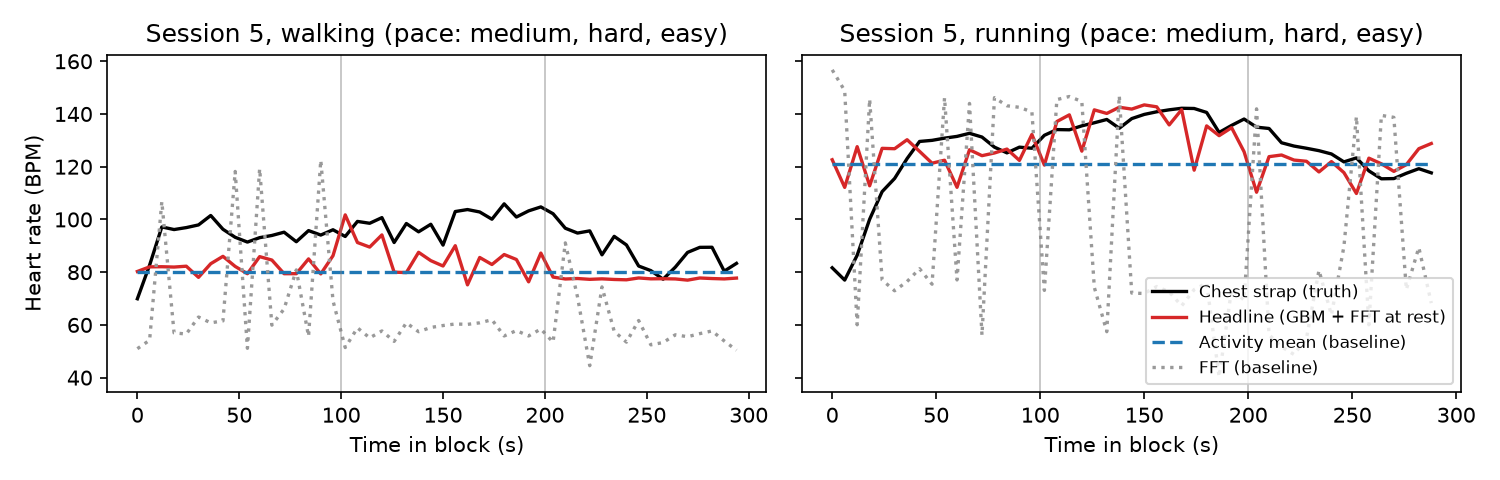
\includegraphics[width=0.92\textwidth]{final_timeseries.png}
\caption{Session 5, the test session: chest-strap heart rate and predictions through the walking and running blocks. Vertical lines mark the pace changes.}
\label{fig:ts}
\end{figure*}

\textbf{What else was tried.} PCA clearly helped: ridge without it scored 11.41~BPM in development, and 8.30 with it. The first component explains 40\% of the variation and is a ``how hard the wrist moves'' axis. I also ran k-means clustering, which groups windows without using labels. With four clusters it recovered the four activities almost exactly, with an adjusted Rand index of 0.95, which explains why Stage~1 is easy. Inside walking, two or three clusters partly followed session~4's pace steps, but inside running they did not. Adding the cluster number as a ``pace level'' input changed development RMSE by less than 0.5~BPM, so it is not used: the clusters mostly repeat the movement intensity the motion features already carry. Two other additions also changed RMSE by less than 0.5~BPM and were dropped: giving the model the FFT estimate as an input, and predicting the difference from the activity mean.

% =============================================================================
\section{Where the Model Fails}
% =============================================================================
\begin{table}[t]
\centering\tsmall
\caption{Session 5 RMSE of the headline by slice. $n$ is windows and $b$ is 5-minute blocks. The 95\% interval resamples whole blocks 2000 times; ``--'' means one block, so no interval.}
\label{tab:slices}
\begin{tabular}{@{}llrrcc@{}}
\toprule
Variable & Slice & $n$ & $b$ & RMSE & 95\% CI \\
\midrule
Heart rate & $\ge$100 & 57 & 2 & 11.8 & [9.0, 19.5] \\
 & $<$100 & 141 & 4 & 8.7 & [2.3, 15.5] \\
Pace step & 0, first 100~s & 34 & 2 & \textbf{16.0} & [12.9, 18.6] \\
 & 1 & 34 & 2 & 12.6 & [8.2, 15.9] \\
 & 2 & 31 & 2 & 11.2 & [9.4, 12.7] \\
Motion, & Q1, still & 50 & 2 & 1.7 & [0.0, 1.7] \\
\texttt{acc\_mag} std & Q2 & 49 & 1 & 2.8 & -- \\
quartile & Q3 & 49 & 1 & 14.0 & -- \\
 & Q4, most motion & 50 & 2 & 13.0 & [8.2, 13.1] \\
Skin contact, & Q1, weak & 50 & 3 & 10.1 & [3.3, 15.9] \\
PPG mean & Q4, strong & 50 & 3 & 6.4 & [1.4, 15.7] \\
Noisy label & strap vs beats $>$5 & 5 & 2 & 8.4 & [5.4, 8.9] \\
\midrule
\multicolumn{2}{@{}l}{\emph{Exploratory:} $<$30~s after pace change} & 20 & 2 & 12.5 & [10.4, 14.3] \\
\bottomrule
\end{tabular}
\end{table}

Table~\ref{tab:slices} splits the session-5 errors by variables that the model does not predict. All of them were fixed before session~5 was run, except the last row, which I added after looking at development data and therefore mark as exploratory. The interval for each slice comes from a block bootstrap: whole 5-minute blocks are resampled, because windows inside a block are not independent.

\textbf{Worst slice: pace step~0}, the first 100~s of the walking and running blocks. RMSE is 16.0~BPM [12.9, 18.6] over 34 windows and 2 blocks. Here heart rate is still climbing from the rest before the block, and the model lags behind (Fig.~\ref{fig:ts}, right). In development the worst slice was the hardest pace step, at 20.2~BPM. Both failures happen where heart rate moves away from the activity's usual level.

\textbf{Other patterns.} Error rises with movement, from 1.7~BPM in the stillest quarter to 13.0 in the most active, and with heart rate, 11.8 above 100~BPM against 8.7 below. It is lower when the sensor touches the skin well, 6.4 against 10.1, though the intervals overlap. The noisy-label slice has only 5 windows, too few to judge. Session~5 has just four blocks, so these slices describe one session rather than prove a general effect.

\textbf{Does the model track heart rate or just the activity?} I subtracted each block's average from both the predictions and the truth and correlated what was left. The headline scores 0.43, ridge 0.09, the FFT $-0.17$, and the activity mean 0, since it is constant inside a block. GBM partly follows real changes within an activity. Ridge mostly just recognises the activity.

% =============================================================================
\section{Recommendation and Future Work}
% =============================================================================
\textbf{Recommendation: use the band for resting and desk work, and keep the chest strap for walking and running.} When still, the band's typical error is 2.3~BPM, 95\% of windows are within 5~BPM, and none read far too low. Unlike the activity mean, it actually measures the pulse at rest, so it would notice a real change in resting heart rate and could feed measures such as a sleep score. While moving, it reads more than 10~BPM too low in 39\% of windows, the error that could push a wearer past their intended effort. It fails any sensible threshold here, not just the one set in Section~I. So a cheap band can work today for the still part of the day, but not yet for exercise.

\textbf{What would reverse it.} I would trust the band during exercise if, on new held-out sessions recorded on other days, fewer than 10\% of moving windows read more than 10~BPM too low and RMSE was near 5~BPM. In the other direction, I would stop trusting it at rest if Stage~1 began calling movement ``resting'', for example a slow walk with a still arm. The FFT would then be used exactly where it fails. So far this happened in 0 of 988 windows.

\textbf{Limitations and future work.}
\begin{itemize}
\item \emph{More people.} All data comes from one person. Skin tone, wrist size, fitness and how the band sits all change the PPG signal. Recording several people and testing on people the model has never seen would show whether it generalises.
\item \emph{Real-world movement.} Every session was in the same room and position, and walking and running were done in place to stay near the laptop. Real running has longer strides, more arm swing and outdoor light. Recording on a treadmill or outdoors, with the band logging to its own memory instead of streaming, would give more realistic data.
\item \emph{The final band.} The prototype was a simple proof of concept, with the boards spread along the forearm and held on by elastic bands. A finished band would hold every sensor in one housing with steadier skin contact, which changes both the PPG and the motion signals. The models would need to be retrained and tested on data collected with that final physical form.
\item \emph{More and longer sessions.} Five sessions, three on one evening, and a test set of only four blocks. The model has seen walking heart rates only up to 106~BPM.
\item \emph{Better signals.} A faster sampling rate and features that remove the arm-swing frequency from the PPG could help the model during motion.
\end{itemize}

\begin{thebibliography}{00}
\bibitem{vicente2023}
J.~M. Vicente-Samper, C.~Tamantini, E.~\'{A}vila-Navarro, M.~\'{A}. De La Casa-Lillo, L.~Zollo, J.~M. Sabater-Navarro, and F.~Cordella, ``An ML-based approach to reconstruct heart rate from PPG in presence of motion artifacts,'' \textit{Biosensors}, vol.~13, no.~7, Art.~no.~718, Jul. 2023, doi: 10.3390/bios13070718.

\bibitem{sklearn}
F.~Pedregosa \textit{et al.}, ``Scikit-learn: Machine learning in Python,'' \textit{J. Mach. Learn. Res.}, vol.~12, pp.~2825--2830, 2011.

\bibitem{claude2026}
Anthropic, ``Claude Opus 5.5,'' 2026. [Online]. Available: \url{https://claude.ai}
\end{thebibliography}

\clearpage
\appendix
\section*{Appendix: AI-Use Note}

\textbf{Tool.} Claude Opus 5.5~\cite{claude2026}, used through Claude Code, an AI coding assistant that reads and edits files in the repository and runs commands. All models were built with scikit-learn~\cite{sklearn}.

\textbf{My work.}
\begin{itemize}
\item \emph{The device.} I chose the parts, wired and mounted the PPG sensor and the board, and built the wrist band.
\item \emph{The data-collection pipeline.} I designed how data is collected: the band and the chest strap streaming to one laptop, one file per activity, and the session protocol with 5-minute blocks and changing pace. I recorded all five sessions and checked each one as it came in.
\item \emph{The ML pipeline.} I chose the two-stage design, the session-based split, the FFT baseline and the model families, based on the literature~\cite{vicente2023} and on comparing Claude's suggestions. I wrote the full pipeline specification, including the slice variables and the rule that session~5 is used once.
\item \emph{The decisions.} The decision framing, adopting the FFT-at-rest rule before the test, and running \texttt{final.py} myself.
\end{itemize}

\textbf{What I asked Claude to do.} Help write and debug the collection code and the Bluetooth pairing, write a collection guide, implement the windowing script and the modelling pipeline from my specification, analyse development results and suggest adjustments, and help draft and edit this report.

\textbf{What it got wrong, and how it was caught.}

\smallskip
{\tsmall
\begin{tabular}{@{}p{0.46\columnwidth}p{0.46\columnwidth}@{}}
\toprule
Error & How caught and fixed \\
\midrule
Assumed the strap would connect without pairing, but it needs an encrypted connection. & The first real test failed with ``Encryption is insufficient''. Added a retry and pairing steps. \\
Counted beats twice: the strap repeats the previous beat times every 0.5~s. & Strap rows came twice per second and the beat lists repeated. Fixed, and the two labels now agree within 1~BPM. \\
Kept windows with no skin contact, where the FFT read about 150~BPM. & The FFT errors were concentrated where the sensor reported no skin. These windows are now dropped. \\
Analysed sessions 4--5 with 2-minute pace steps, but the protocol used 100~s. & Step cadence from the band jumps at 100 and 200~s. Corrected in \texttt{label.py}. \\
The tuning loop fitted on arrays but predicted on tables. & scikit-learn warnings. Fixed, with no change in RMSE. \\
\texttt{final.py} used a function needing an uninstalled package, so the one-time run would have crashed. & Code review before a practice run. Replaced and tested on a stand-in split, training on 1--3 and testing on 4. \\
In that practice run, the test script returned session-5 rows. & An assertion stopped it before any computation. Session 5 stayed unused until \texttt{final.py}. \\
A generated sentence overstated a k-means result. & Read against the numbers next to it and reworded. \\
\bottomrule
\end{tabular}}

\smallskip
\textbf{What I verified myself.} The FFT baseline matches my earlier hand-checked numbers, 27.85~BPM on sessions 1--3 and 2.01 at rest. Window counts are 49 to 50 per block. A leakage check confirms no session-5 row was loaded before \texttt{final.py}. The full log is in \texttt{AI\_LOG.md}.

\end{document}
